% ----------------------------------------------------------
% Metodologia
% ----------------------------------------------------------
\chapter{Metodologia}
\label{chap:metodologia}

O trabalho de tese em questão trata-se, essencialmente, do desenvolvimento e testes
de um sistema de \textit{software}. Desse modo, parece desejável, do ponto de vista de
clareza, descrever a metodologia utilizada no trabalho de forma a acompanhar o ciclo
de desenvolvimento dos vários elementos de software utilizados. Para isso, a metodologia
será divida em seções, da seguinte forma:

\section{Visão Geral}

\begin{figure}[htb]
  \caption{Metodologia: o sistema acoplado.}
  \centering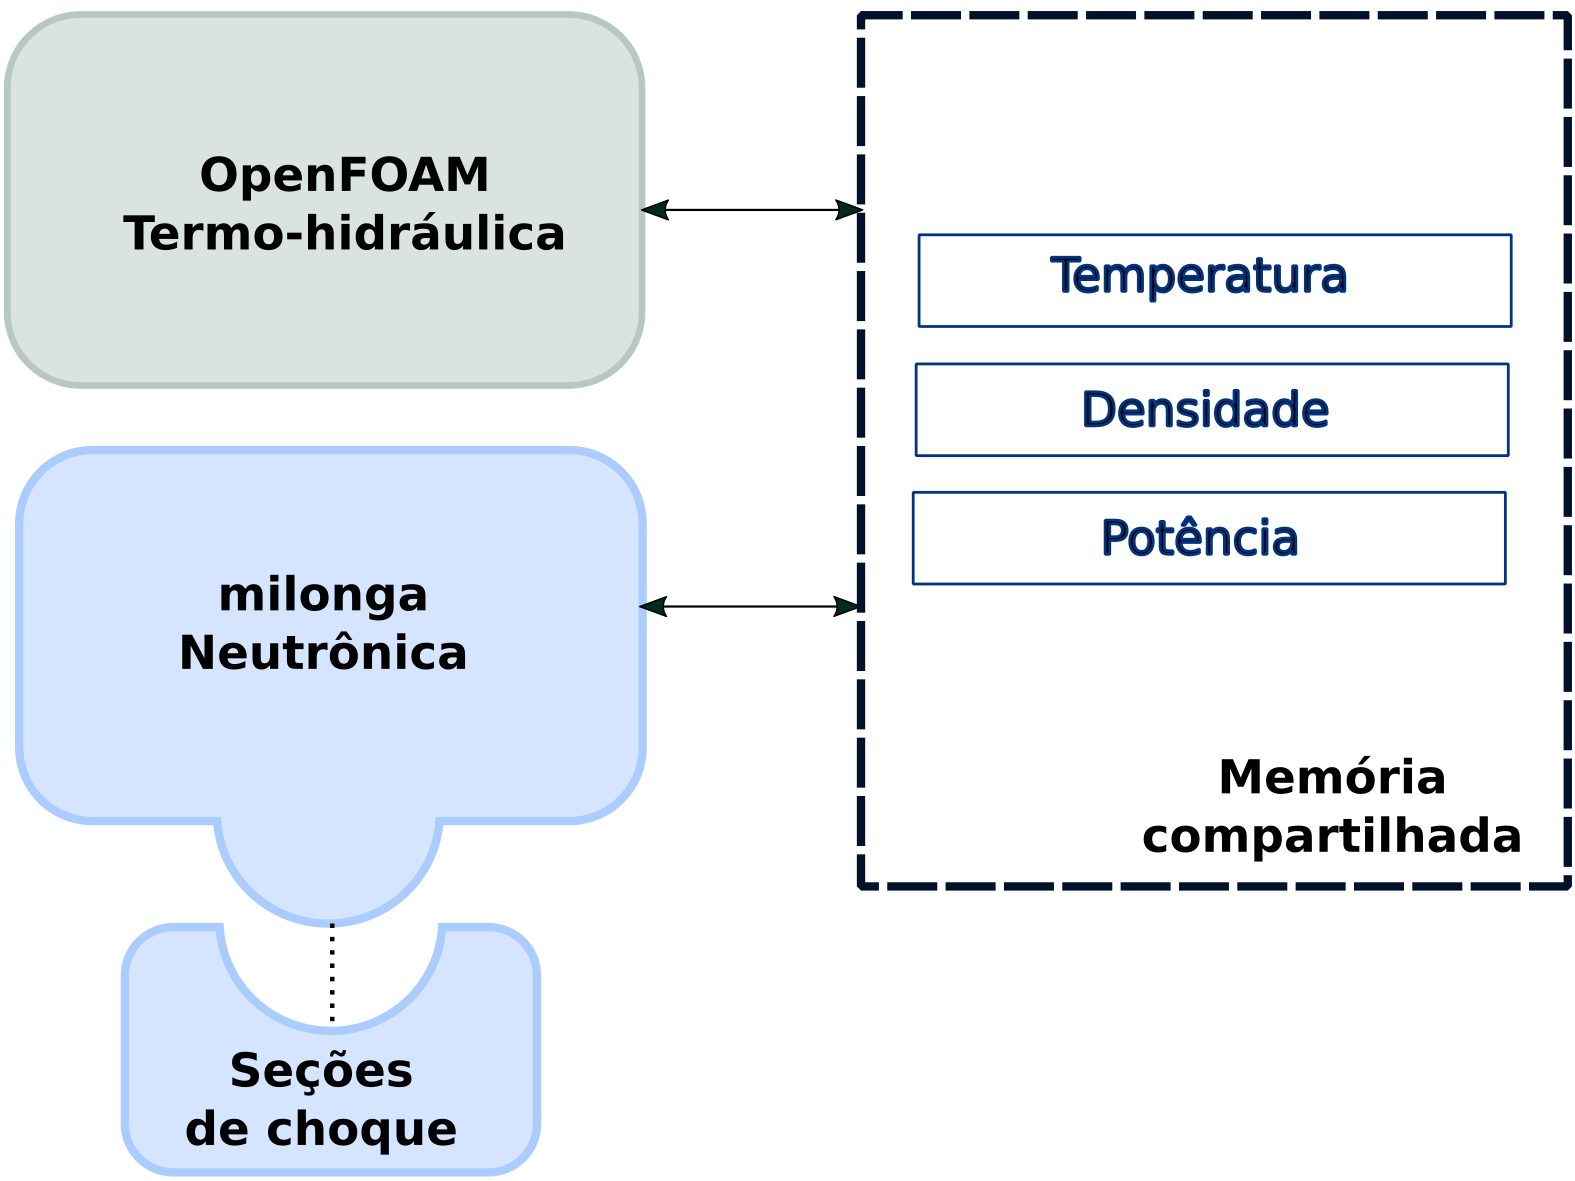
\includegraphics[scale=0.7]{figuras/metodologia1.png}
  \label{metodoetapas}
  \legend{Fonte: autor}
\end{figure}

\section{\textit{Shared-memory}}

É desconhecido na literatura o uso de memória compartilhada (\textit{shared-memory} para
acoplamento neutrônico e termo-hidráulico.


\section{Ferramentas}
\label{sec:ferr}

\subsection{Termo-hidráulica: \textit{OpenFOAM}}
\label{subsection:openfoam}


\subsection{Neutrônica: \textit{milonga}}
\label{subsection:milonga}


% *******************************************************************
\section{Estruturas de dados}

\begin{itemize}
\item Alteração de hash para vetor (1 parágrafo)
\item 1 parágrafo para a criação de Q
\item Criação de vetores shared-memory e semáforos
\end{itemize}

1 parágrafo: preparação para rodar em paralelo. Divisão externa ao OpenFOAM, por isso não foi
implementado. Ficou para trabalhos futuros. Até porque precisa do milonga também paralelizado.

\subsection{Equações}

\begin{itemize}
\item Adição do termo-fonte (1 alteração na equação do sólido: colocar equação já no formato OpenFOAM)
\end{itemize}

\subsection{Malha}

\begin{figure}[htb]
  \caption{Malha e regiões, vista superior.}
  \centering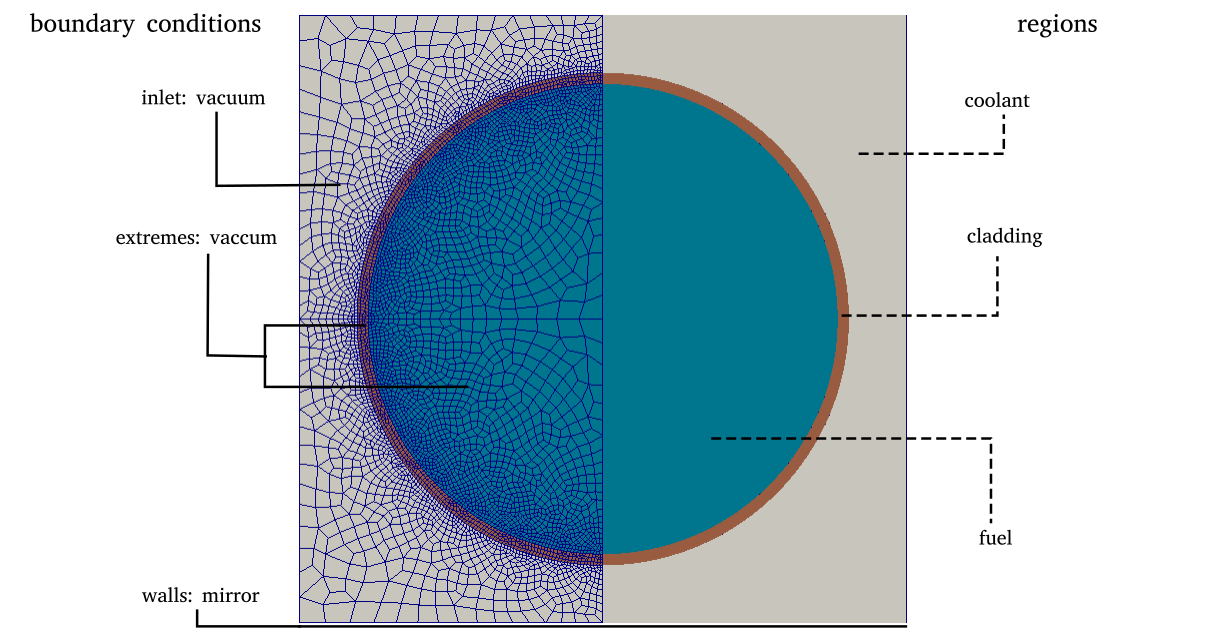
\includegraphics[scale=0.5]{figuras/regions_neutronica_malha_e_sem.png}
  \label{regions_malha}
  \legend{Fonte: autor}
\end{figure}

\subsection{Condições de contorno}


\section{Acoplamento} % Algoritmos

\subsection{Algoritmo neutrônica}

\begin{figure}[htb]
  \caption{Algoritmo neutrônica.}
  \centering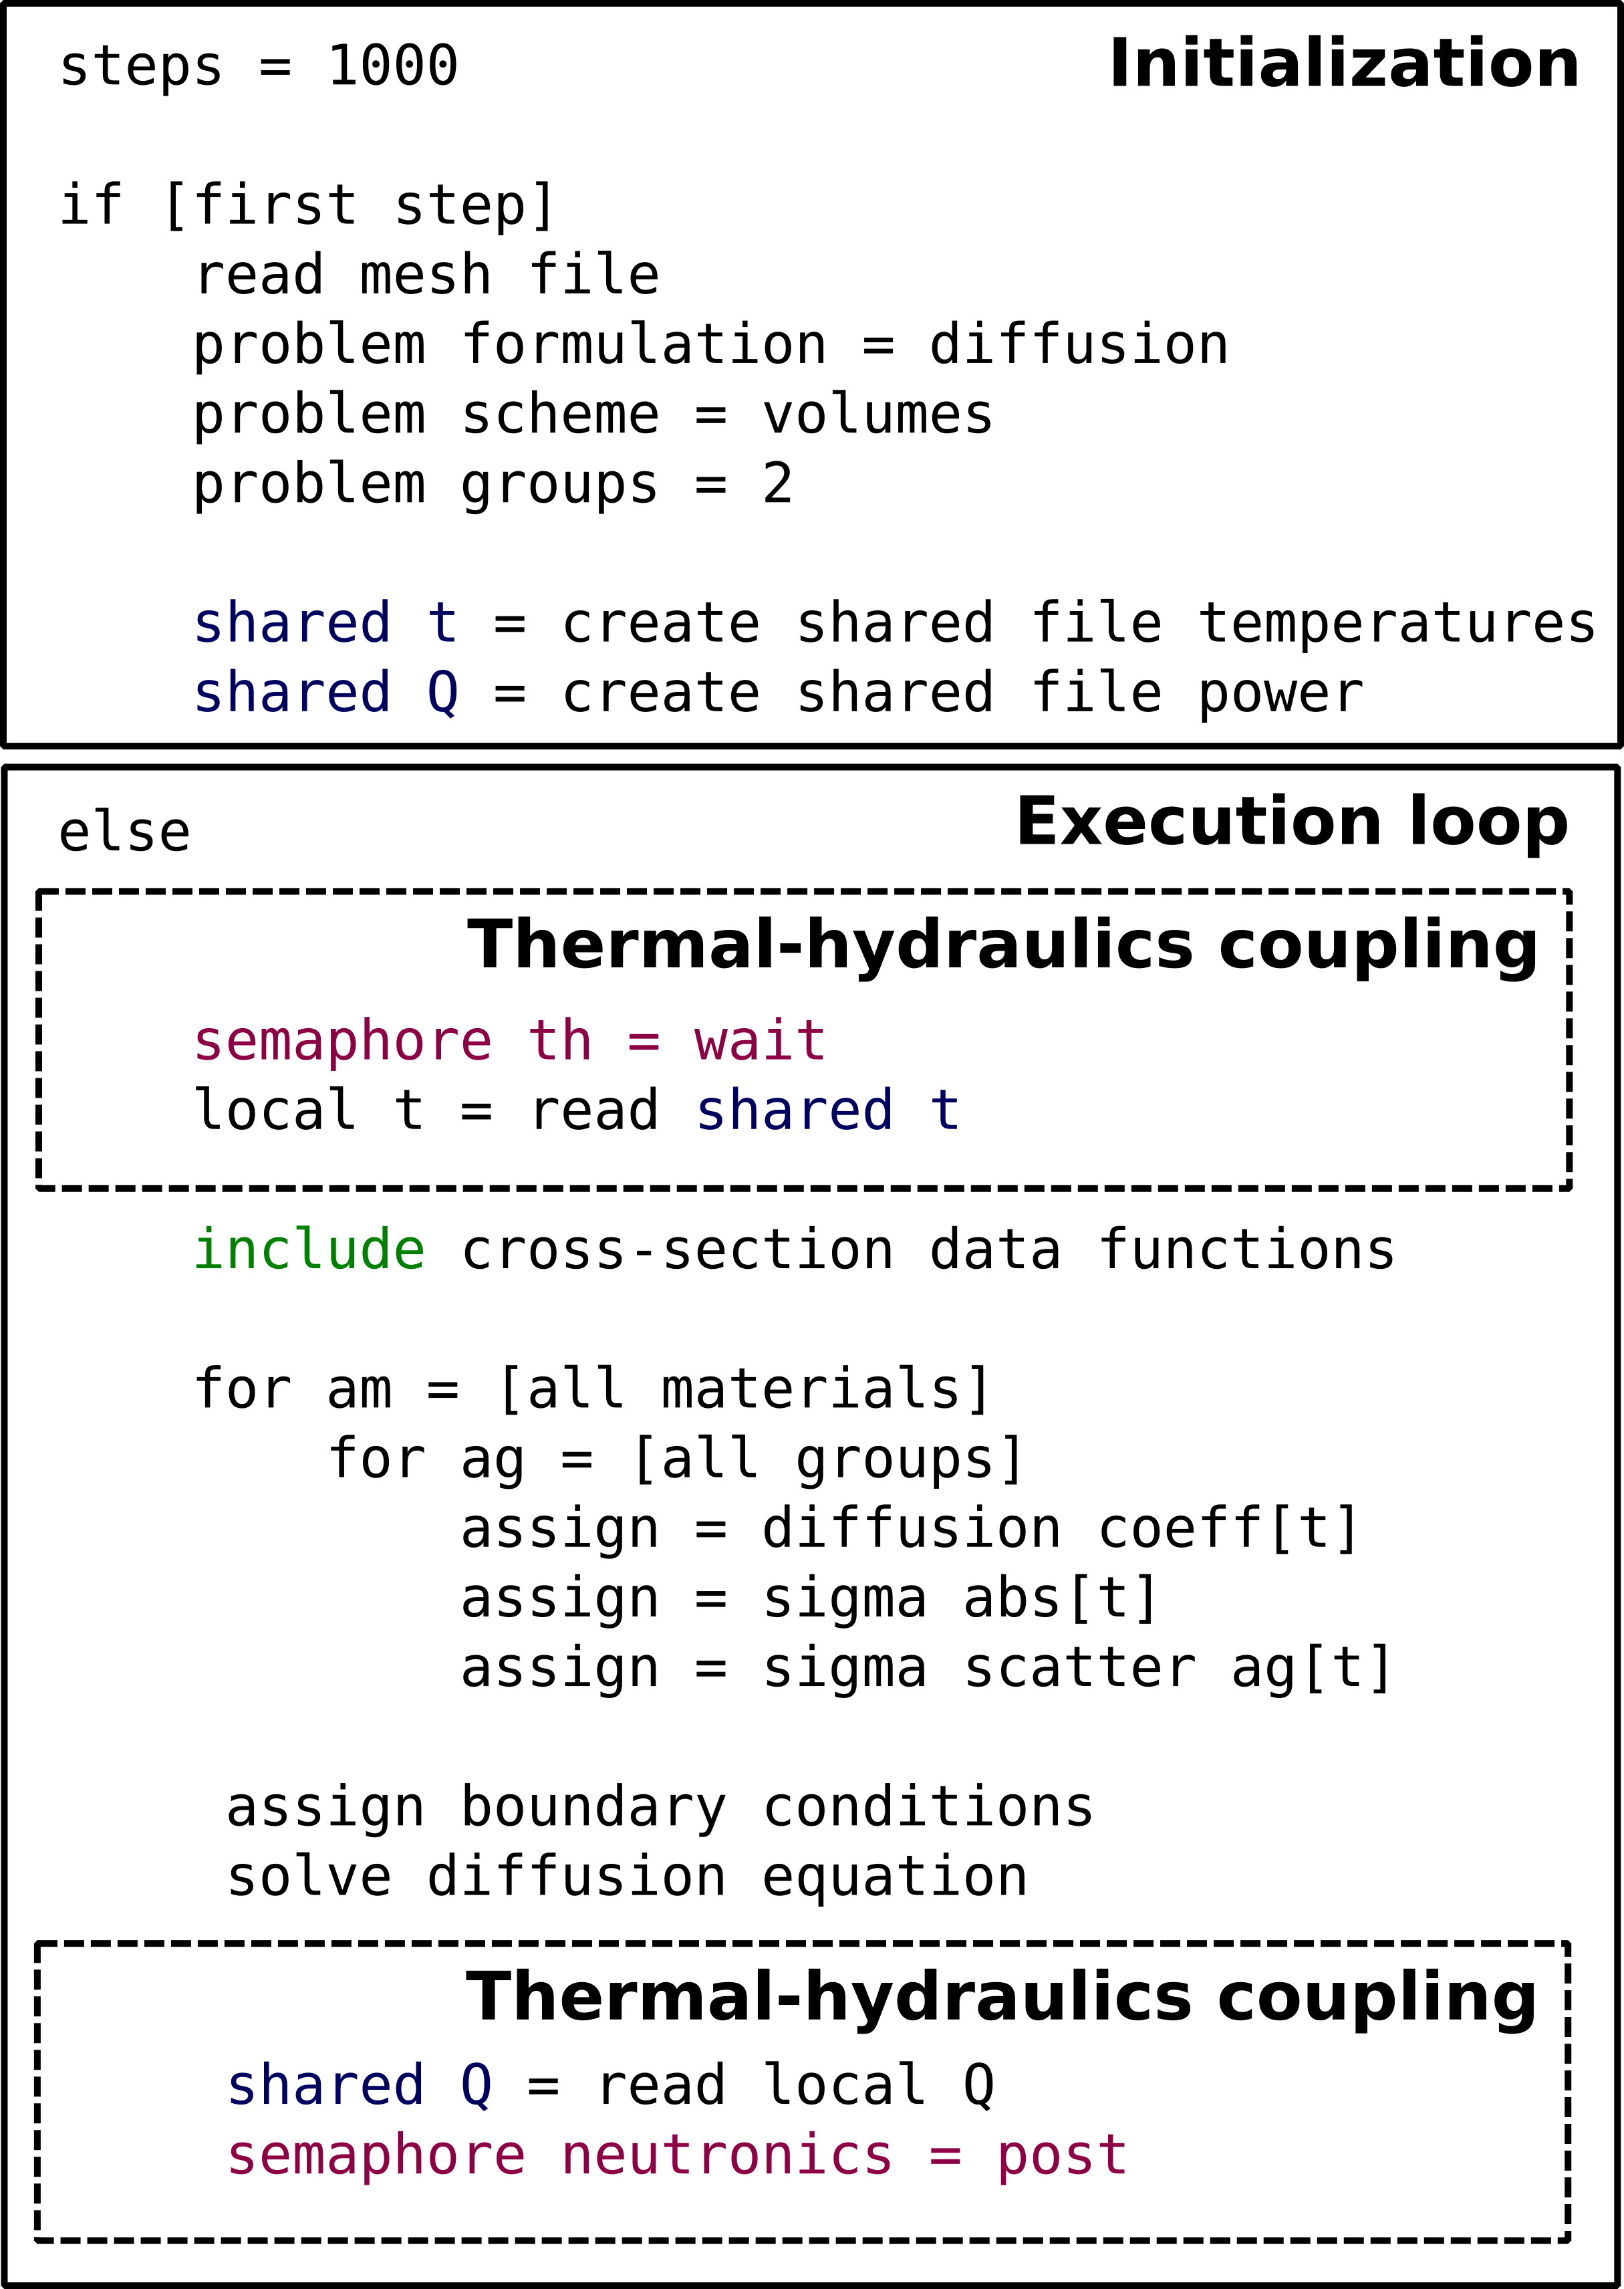
\includegraphics[scale=0.5]{figuras/algoritmos_milonga.png}
  \label{algo_neutronica}
  \legend{Fonte: autor}
\end{figure}

\subsection{Algoritmo termo-hidráulica}
\label{subsec:th}

\begin{figure}[htb]
  \caption{Algoritmo termo-hidráulica.}
  \centering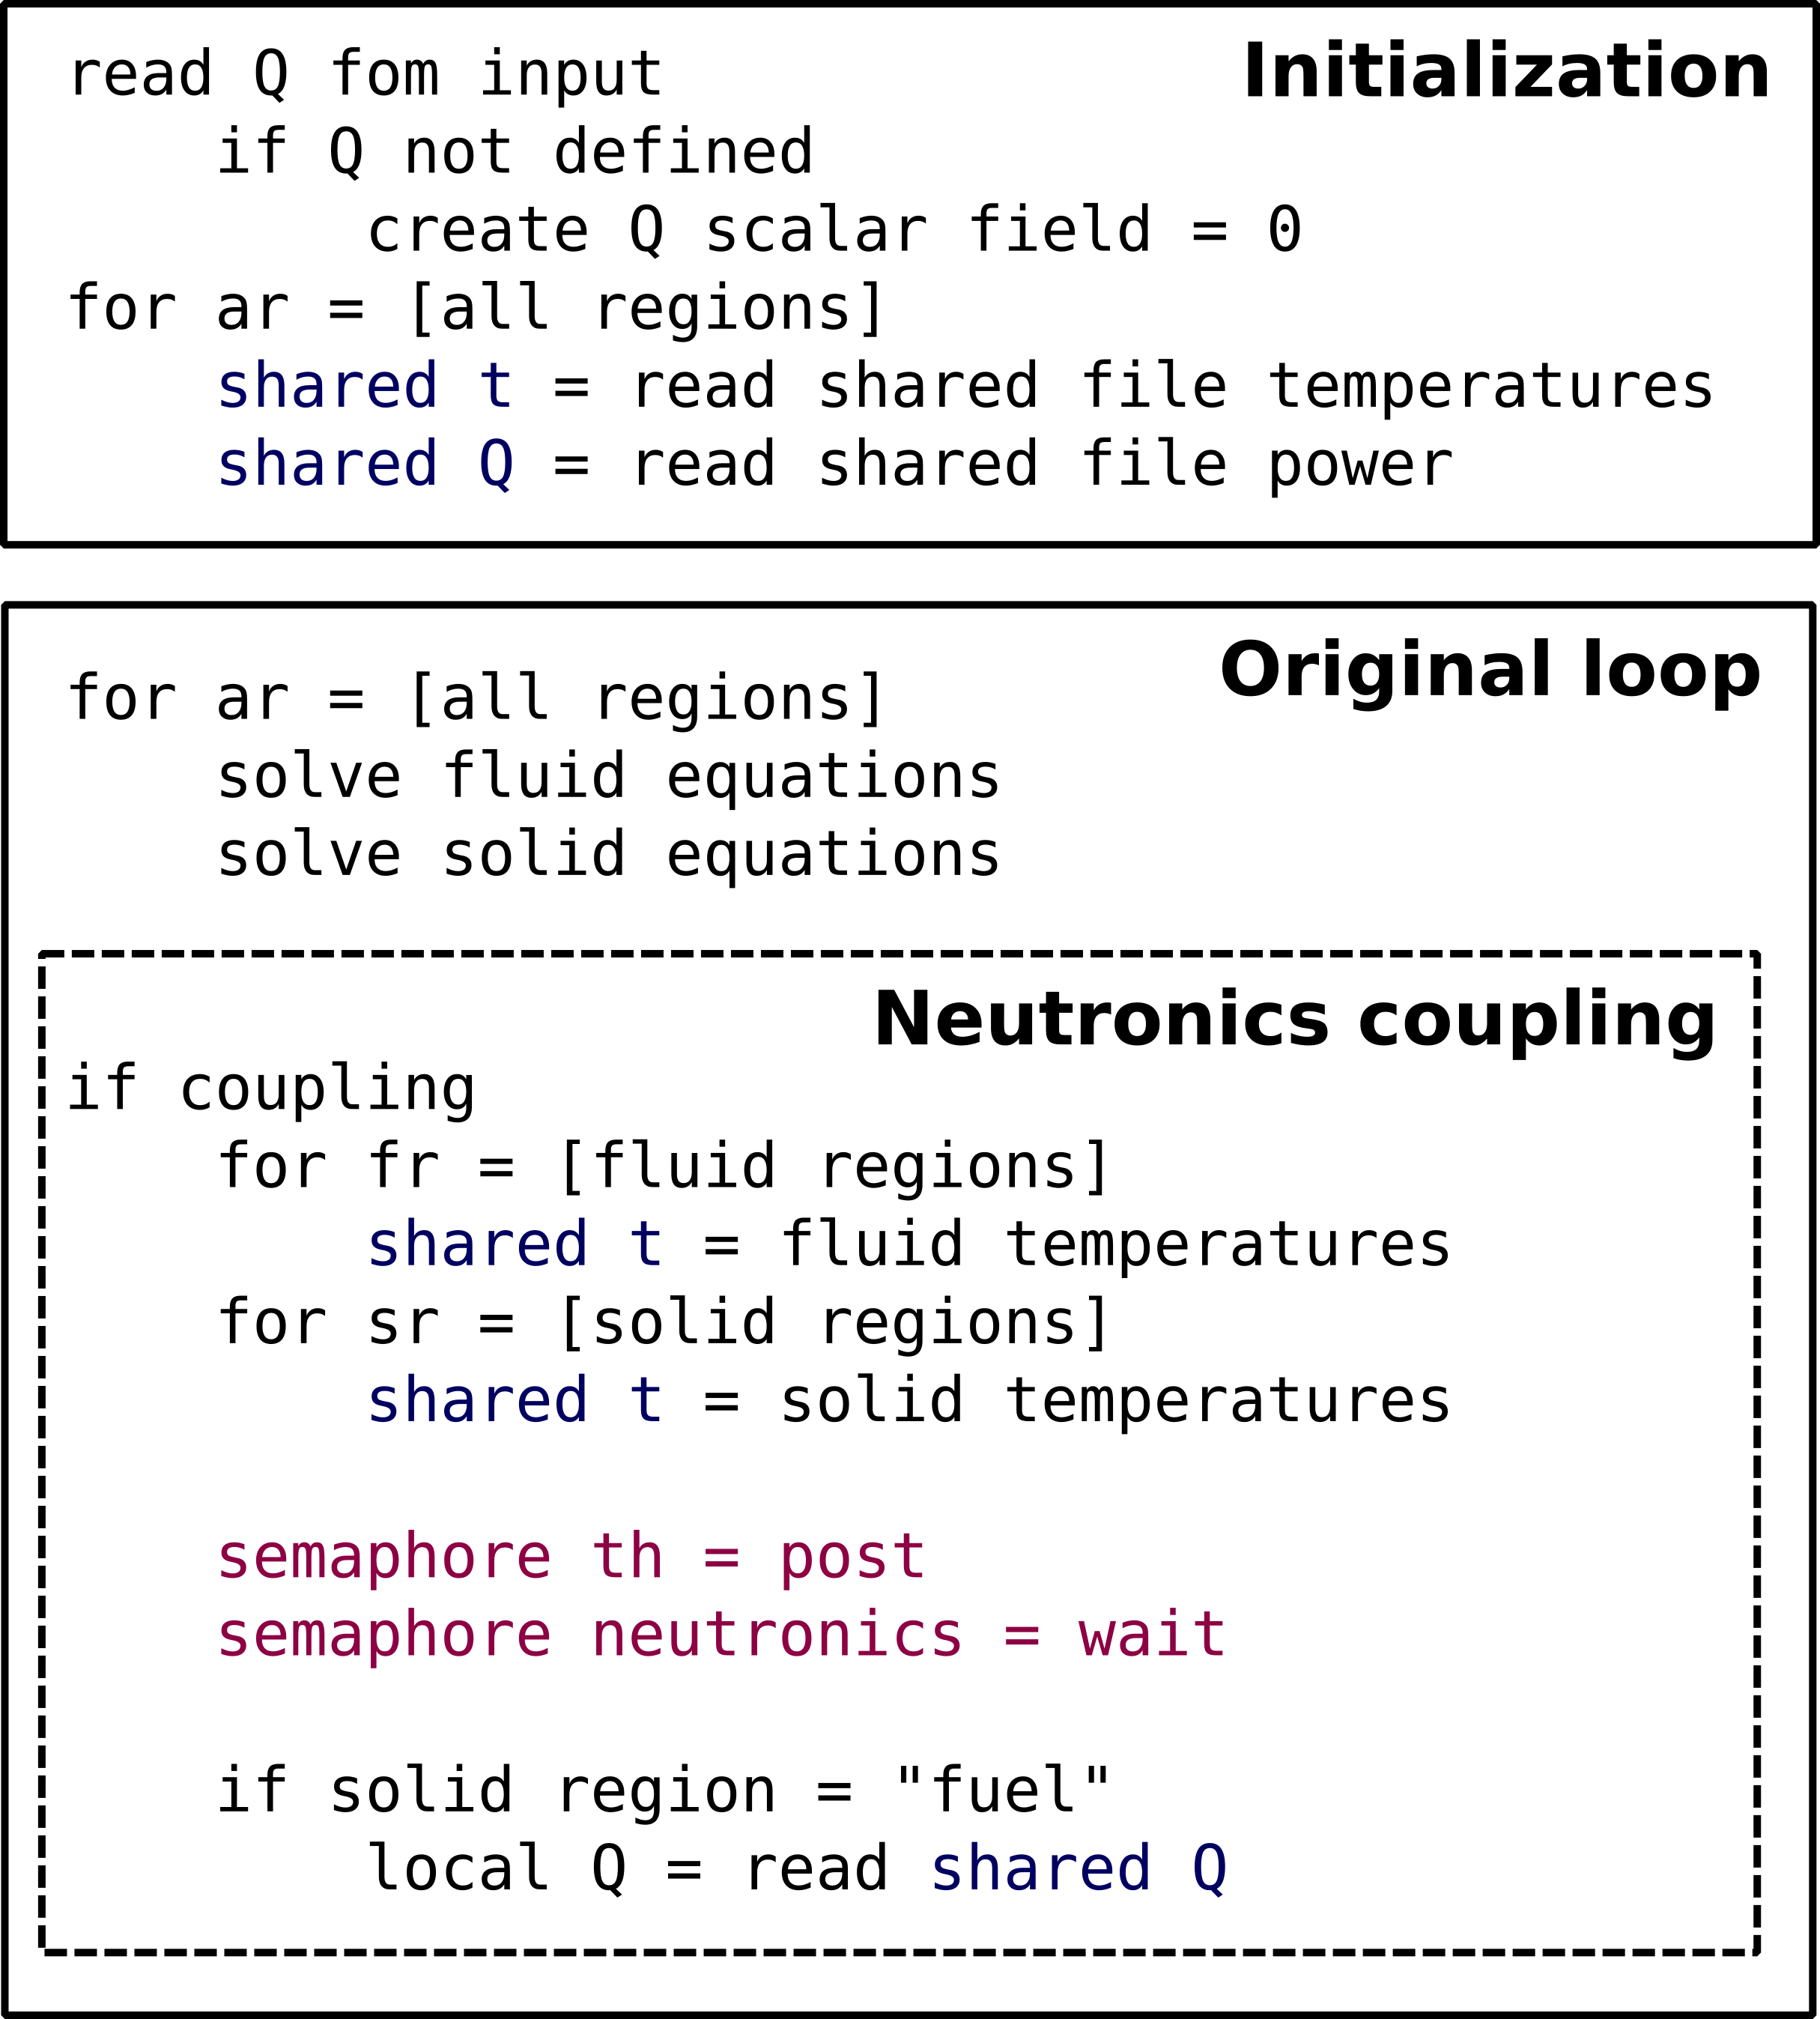
\includegraphics[scale=0.5]{figuras/algoritmo_openfoam.png}
  \label{algo_th}
  \legend{Fonte: autor}
\end{figure}



%Modelada uma geometria idêntica à representada na malha utilizada pelo \textit{OpenFOAM},
%foram feitas simulações da neutrônica pelo Serpent com objetivo de obter as seções
%de choque em dois grupos a serem usadas na solução da aproximação por difusão dos nêutrons
%pelo \textit{milonga}.

%Na saída do Serpent são dados constantes de groups homogeneizadas (neste caso, com espectro
%corrigido para fugas pelo método B1 \textbf{CITAR}) e outros parâmetros de interesse para
%a modelagem por difusão como, por exemplo, os coeficientes de difusão para cada grupo já
%calculados.

%Como todos os elementos do desenvolvimento estão relacionados entre si, sempre que
%julgado oportuno para a clareza do entendimento, os conceitos desenvolvidos em cada
%seção poderão ser apresentados conjuntamente. De fato, uma vez que o problema multifísica
%(ou acoplamento) nada mais é do que a solução conjunta de dois problemas que são,
%usualmente, resolvidos separadamente, é natural como definir, modelar e resolver os
%dois problemas separadamente.

%De acordo com as definições de problemas acoplados apresentadas
%no capítulo \ref{chap:rev}, ao resolver os problemas neutrônico e termo-hidráulico
%separadamente, o acoplamento ainda pode ser considerado implícito de acordo com, já que a troca de informações entre os problemas ocorre ao nível de termos completos,
%e não em condições de contorno. É importante dizer que essa nomeclatura para as formas
%de acoplamento não é unânime na literatura \cite{Ivanov2007}.

%Deve estar claro que a metodologia a ser descrita trata do ciclo de desenvolvimento
%do \textit{software} acoplado. Apesar de ser possível considerar as simulações e
%os processos de pré-processamento e pós-processamento, tanto termo-hidráulicos quanto
%neutrônicos, optou-se por tratar destas etapas exclusivamente na seção de validação e,
%quando pertinente, nos resultados obtidos.


%Na figura \ref{metodoetapas} são apresentadas as relações entre os diferentes elementos
%do sistema acoplado.





